\documentclass[crop=false]{standalone}
\usepackage{circuitikz}
\usepackage{tikz}
\usetikzlibrary{positioning}

\begin{document}
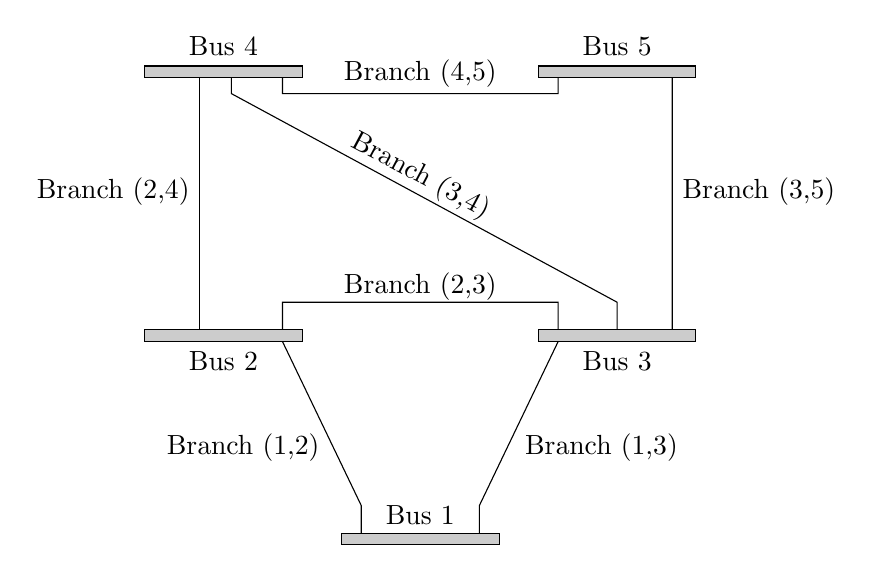
\begin{tikzpicture}
\draw (-0.8,-0.35) to [short] (-0.8,3); %branch 2,4
\draw (-0.4,3) to [short] (-0.4,2.65) to [short]  (4.5,0) to [short]  (4.5,-0.35);  %branch 3,4
\draw (0.25,-0.35) to [short] (0.25,0) to [short]  (3,0) to [short] (3.75,0) to [short] (3.75,-0.35); %branch 2,3
\draw (3.75,-0.5) to [short] (2.75,-2.582) to [short] (2.75,-2.932); %branch 1,3
\draw (0.25,-0.5) to [short] (1.25,-2.582) to [short] (1.25,-2.932); % branch 1,2
\draw (5.2,-0.5) to [short] (5.2,3); %branch 3,5
\draw (0.25,3) to [short] (0.25,2.65) to [short]  (3.75,2.65) to [short] (3.75,3); %branch 4,5



\filldraw[fill=black!20!white, draw=black] (-1.5,3) rectangle (0.5,2.85); %bus 4
\filldraw[fill=black!20!white, draw=black] (-1.5,-0.5) rectangle (0.5,-0.35); %bus 2
\filldraw[fill=black!20!white, draw=black] (3.5,-0.5) rectangle (5.5,-0.35); %bus 3
\filldraw[fill=black!20!white, draw=black] (1,-3.082) rectangle (3,-2.932); %bus 1
\filldraw[fill=black!20!white, draw=black] (3.5,3) rectangle (5.5,2.85);%bus 5


\node[align=left] at (2,-2.7) {Bus 1};
\node[align=left] at (-.5,-0.75) {Bus 2};
\node[align=left] at (4.5,-0.75) {Bus 3};
\node[align=left] at (-.5,3.25) {Bus 4};
\node[align=left] at (4.5,3.25) {Bus 5};

\node[align=left] at (4.3,-1.85) {Branch (1,3)};
\node[align=left] at (-0.25,-1.85) {Branch (1,2)};
\node[align=left] at (2,0.2) {Branch (2,3)};
\node[align=left] at (2,2.9) {Branch (4,5)};
\node[align=left,rotate=-28] at (2,1.6) {Branch (3,4)};
\node[align=left] at (-1.9,1.4) {Branch (2,4)};
\node[align=left] at (6.3,1.4) {Branch (3,5)};


\end{tikzpicture}

\end{document}